%!TeX spellcheck = en-US
%!TEX root = ../hw3_report.tex
We implement the naive approach for solving the Lyapunov equation and compare it to the Bartels-Stewart method on random matrices. The dependence of the simulation time on $n$ is illustrated in Figure \ref{task1}. Theoretically, the complexity is as bad as $\mathcal O(n^6)$ for the naive approach and $\mathcal O(n^3)$ for the improved algorithm. However, the simulation time is in this test smaller due to the use of improved linear solvers in Matlab. Tests were done with the Matlab \texttt{timeit} command and the system was solved 10 times for each matrix size, such that an avarage computation time could be determined. From our investigations, we conclude that the theoretical complexities should be seen as upper bounds for the complexity. The measured complexity is $\mathcal O(n^{4.30})$ and $\mathcal O(n^{1.80})$  respectively (if fitted to a straight line in the loglog-plot) and $\mathcal O(n^{4.38})$ and $\mathcal O(n^{1.76})$ if the \texttt{cputime} command is used for the measurements instead. 
\todo{Fredrik: kan du förklara komplexiteten bättre?}
\begin{figure}[h!]
\centering
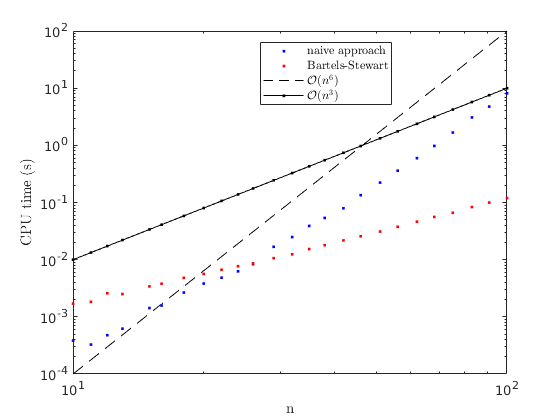
\includegraphics[scale=0.5]{cpu.png}
\caption{Measured CPU-time for solving the Lyapunov equation on random matrices of size $n$ using a naive appoach compared to the Bartels-Stewart algorithm.}
\label{task1}
\end{figure}

\begin{figure}[h!]
\centering
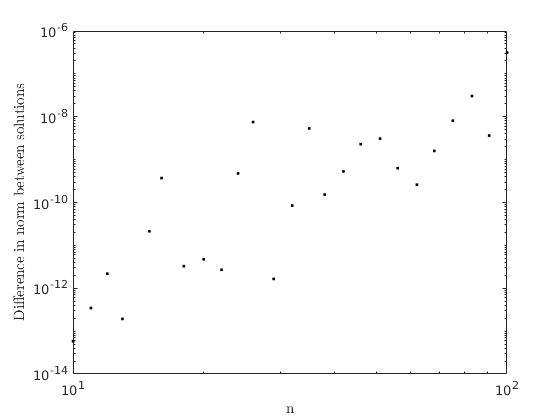
\includegraphics[scale=0.5]{norm.png}
\caption{Difference in norm between the naive approach and the Bartels-Stewart algorithm for soving the Lyapunov equation on random matrices of size $n$.}
\label{task1}
\end{figure}


